\documentclass[12pt, twoside]{article}
\usepackage[letterpaper, margin=1in, headsep=0.2in]{geometry}
\setlength{\headheight}{0.6in}
%\usepackage[english]{babel}
\usepackage[utf8]{inputenc}
\usepackage{microtype}
\usepackage{amsmath}
\usepackage{amssymb}
%\usepackage{amsfonts}
\usepackage{siunitx} %units in math. eg 20\milli\meter
\usepackage{yhmath} % for arcs, overparenth command
\usepackage{tikz} %graphics
\usetikzlibrary{quotes, angles}
\usepackage{graphicx} %consider setting \graphicspath{{images/}}
\usepackage{parskip} %no paragraph indent
\usepackage{enumitem}
\usepackage{multicol}
\usepackage{venndiagram}

\usepackage{fancyhdr}
\pagestyle{fancy}
\fancyhf{}
\renewcommand{\headrulewidth}{0pt} % disable the underline of the header
\raggedbottom
\hfuzz=2mm %suppresses overfull box warnings

\usepackage{hyperref}

\fancyhead[LE]{\thepage}
\fancyhead[RO]{\thepage \\ Name: \hspace{4cm} \,\\}
\fancyhead[LO]{BECA / Dr. Huson / Geometry\\*  Unit 1: Segments, length, and area\\* 19 Sept 2022}

\begin{document}

\subsubsection*{1.8 Classwork: Area of rectangles, triangles, parallelograms}
\begin{enumerate}

\item Find the \emph{area} of the shape shown below composed of a rectangle and two semi-circular caps. Leave your answer as an exact value in terms of $\pi$.
\begin{flushright}
\begin{tikzpicture}[scale=.635]
  \draw[help lines] (-1,-1) grid (7,7);
  \draw[thick, ->] (-1.2,0) -- (7.4,0) node [below right] {$x$};
  \draw[thick, ->] (0,-1.2)--(0,7.4) node [left] {$y$};
  \draw[thick] (2,2)--(5,2)--(5,4)--(2,4)--cycle;
  \draw[thick] (2,4) arc (90:270:1);
  \draw[thick] (5,2) arc (-90:90:1);
\end{tikzpicture}
\end{flushright}




\newpage
\item A square is partitioned into two rectangles. The sum of the perimeters of the two rectangles is 36. Find the area of the square.
\begin{flushright}
\begin{tikzpicture}%[scale=.635]
  \draw [thick]  (0,0) rectangle (6,6);
  \draw [thick] (0,4)--(6,4);
\end{tikzpicture}
\end{flushright}


\item Find the circumference of the earth's orbit around the sun. \vspace{2cm}

 
\item Spicy: Find the area of the $\triangle ABC$ is shown below with $A(3,2)$, $B(7,4)$, and $C(4,8)$. 
  \begin{multicols}{2}
    \begin{enumerate}
      \item First find the area of the red rectangle with sides $b=4$, $h=6$.
      \item Find the area of the three triangles surrounding $\triangle ABC$ in the rectangle. 
      \item Subtract their areas from the rectangle to find $A_{\triangle ABC}$
      \end{enumerate}
      \begin{flushright}
      \begin{tikzpicture}[scale=.635]
        \draw[help lines] (-1,-1) grid (9,9);
        \draw[thick, ->] (-1.2,0) -- (9.4,0) node [below right] {$x$};
        \draw[thick, ->] (0,-1.2)--(0,9.4) node [left] {$y$};
        %\draw[<->, thick] (0.5,1)--(0.5,5);
        \draw[thick] (3,2)--(7,4)--(4,8)--cycle;
        \draw[thick, red] (3,2)--(7,2)--(7,8)--(3,8)--cycle;
        \draw[fill] (3,2) circle [radius=0.05] node[below left] {$A$};
        \draw[fill] (7,4) circle [radius=0.05] node[right] {$B$};
        \draw[fill] (4,8) circle [radius=0.05] node[above right] {$C$};
        \node at (5,2)[below]{$4$};
        \node at (2.2,5)[right]{$6$};
      \end{tikzpicture}
      \end{flushright}
  \end{multicols} 
  
\item Given $\overline{ABC}$, $AB=\frac{2}{3}$, and $AC=3 \frac{1}{3}$. \par \smallskip
  Find ${BC}$. \par \smallskip
  \begin{tikzpicture}
    \draw[thick] (1,0)--(7,0);
    \draw[fill] (1,0) circle [radius=0.05] node[below]{$A$};
    \draw[fill] (2,0) circle [radius=0.05] node[below]{$B$};
    \draw[fill] (7,0) circle [radius=0.05] node[below]{$C$};
  \end{tikzpicture} \vspace{2cm}

\item Given $\overline{DEFG}$, $DE=3 \frac{1}{4}$, $EF=6 \frac{1}{4}$, and $FG= 1 \frac{3}{4}$. (diagram not to scale) \par \smallskip
Find ${DG}$, expressed as a fraction, not a decimal. \vspace{1cm}
  \begin{flushleft}
    \begin{tikzpicture}
      \draw[thick] (0,0)--(9,0);
      \draw[fill] (0,0) circle [radius=0.05] node[below]{$D$};
      \draw[fill] (3,0) circle [radius=0.05] node[below]{$E$};
      \draw[fill] (7,0) circle [radius=0.05] node[below]{$F$};
      \draw[fill] (9,0) circle [radius=0.05] node[below]{$G$};
    \end{tikzpicture}
  \end{flushleft} \vspace{2cm}
  
\item Given $\overline{FGHI}$, $FG=8 \frac{1}{6}$, $GH=12 \frac{1}{3}$, and $HI= 5 \frac{1}{2}$. (diagram not to scale) \par \smallskip
Find ${FI}$. \par \bigskip
  \begin{tikzpicture}
    \draw[thick] (0,0)--(9,0);
    \draw[fill] (0,0) circle [radius=0.05] node[below]{$F$};
    \draw[fill] (3,0) circle [radius=0.05] node[below]{$G$};
    \draw[fill] (7,0) circle [radius=0.05] node[below]{$H$};
    \draw[fill] (9,0) circle [radius=0.05] node[below]{$I$};
  \end{tikzpicture} \vspace{1cm}

\item Given $\overleftrightarrow{JK}$ as shown on the number line. \par \smallskip
  \begin{tikzpicture}[scale=0.5]
    \draw[<->] (49,0)--(71,0);
    \foreach \x in {50, 52,...,70}
      \draw[shift={(\x,0)}] (0pt,-6pt)--(0pt,6pt) node[below=5pt]{$\x$};
    \draw[fill] (54,0) circle [radius=0.1] node[above]{$J$};
    \draw[fill] (68,0) circle [radius=0.1] node[above]{$K$};
  \end{tikzpicture} \par \bigskip
  What is the midpoint between the points $J$ and $K$? \vspace{2cm}

  \item The point $M(2.3)$ is the midpoint of segment $\overline{AB}$. Given $A(-1.5)$, find the value of $B$. Mark and label it below. \par \smallskip
  \begin{tikzpicture}
    \draw[<->] (-2.5,0)--(8.5,0);
    \foreach \x in {-2,...,8}
      \draw[shift={(\x,0)}] (0pt,-3pt)--(0pt,3pt) node[below=5pt]{$\x$};
    \draw[fill] (-1.5,0) circle [radius=0.05] node[above]{$A(-1.5)$};
    \draw[fill] (2.3,0) circle [radius=0.05] node[above]{$M(2.3)$};
  \end{tikzpicture} \vspace{2cm}

\item Given $\overleftrightarrow{RS}$ as shown on the number line, with $R=-2.8$ and $S=4.4$. \par \smallskip
  \begin{tikzpicture}
    \draw[<->] (-4.5,0)--(6.5,0);
    \foreach \x in {-4,...,6} %2 leading for diff!=1
      \draw[shift={(\x,0)},color=black] (0pt,-3pt) -- (0pt,3pt) node[below=5pt]  {$\x$};
      \draw[fill] (-2.8,0) circle [radius=0.05] node[above]{$R$};
      \draw[fill] (4.4,0) circle [radius=0.05] node[above]{$S$};
  \end{tikzpicture} \par \smallskip
  The points $T$ and $U$ trisect $\overline{RS}$. Find their values, and mark and label them on the number line. \vspace{2cm}
  
\item Given $\overline{PQR}$, with $PQ=\frac{1}{2} x+4$, $QR=x+3$, and $PR=2x+5$. Find ${PR}$. \vspace{2cm}

\end{enumerate}
\end{document}